\documentclass[main.tex]{subfiles}
\begin{document}


\chapter{Examenvragen}
\label{cha:examenvragen}


\begin{examenvraag}{Tussentijdse Toets 2014}
  \begin{ex-vraag}
  Zij $\Omega$ een niet-aftelbare verzameling en zij $\mathcal{A}$ de volgende verzameling:
  \[ \mathcal{A} = \{ A \in \Omega \mid A \text{ is aftelbaar} \vee A^{C} \text{ is aftelbaar } \} \]
  Bewijs dat $\mathcal{A}$ een $\sigma$-algebra is.
  \end{ex-vraag}

  \begin{ex-antwoord}
    \begin{proof}
      \kennen{We gaan eenvoudigweg alle definierende eigenschappen van een $\sigma$-algebra af:}
      \begin{itemize}
      \item $\Omega \in \mathcal{A}$\\
        $\Omega^{C}$ is leeg en dus aftelbaar, dus $\Omega$ zit in $\mathcal{A}$.
      \item $\forall A \in \mathcal{A}: A^{C}\in \mathcal{A}$\\
        Kies een willekeurige $A \in \mathcal{A}$. 
        We onderscheiden twee gevallen.
        \begin{itemize}
        \item $A$ is aftelbaar: $A^{C}$ zit dan in $\mathcal{A}$ want $A^{C^{C}} = A$ is aftelbaar.
        \item $A^{C}$ is aftelbaar: $A$ zit dan in $\mathcal{A}$ want $A^{C}$ is aftelbaar.
        \end{itemize}
      \item $\forall (A_{n})_{n}, A\in \mathcal{A}: \bigcup_{n} A_{n} \in \mathcal{A}$\\
        Fixeer een rij $(A_{n})_{n}$ in $\mathcal{A}$.
        We onderscheiden opnieuw twee gevallen.
        \begin{itemize}
        \item Alle $A_{n}$ zijn aftelbaar: $\bigcup_{n}A_{n}$ is dan aftelbaar en zit dus in $\mathcal{A}$.
        \item Er is minstens \'e\'en $A_{n}$ niet aftelbaar. Opdat die $A_{m}$ in $\mathcal{A}$ zou zitten moet $A_{m}^{C}$ aftelbaar zijn.
          $\left(\bigcup_{n}A_{n}\right)^{C} = \bigcap_{n}A_{n}^{C}$ is nu aftelbaar omdat $A_{m}$ aftelbaar is.
          Bijgevolg zit $\bigcup_{n}A_{n}$ ook in $\mathcal{A}$.
        \end{itemize}
      \end{itemize}
    \end{proof}
  \end{ex-antwoord}
\end{examenvraag}

\begin{examenvraag}{Tussentijdse Toets 2015}
  \begin{ex-vraag}
    Beschouw een systeem dat bestaat uit 4 onafhankelijke componenten $A$, $B$, $C$ en $D$.
    De component $C$ staat in serie met $B$ en zij staan in parallel met $A$.
    Dit systeem staan dan op zijn beurt in serie met $D$.
    De faalkansen van $A$, $C$ en $D$ zijn gekend: $p_{A} = 0.05$, $p_{C}=0.02$, $p_{D}=0.01$.
    Wat is de faalkans van $B$ als we weten dat de kans dat $B$ faalt gegeven dat het hele systeem $S$ faalt gelijk is aan $0.1$?
  \end{ex-vraag}

  \begin{ex-antwoord}
    \begin{itemize}
    \item Definities:
      \begin{itemize}
      \item Noem $p_{i}$ de kans dat systeem $i$ faalt.
      \item Noem $E$ het serieel systeem van $B$ en $C$
      \item Noem $F$ het parallel systeem van $A$ en $E$.
      \item Noem $S$ het hele systeem, dus het seriele systeem van $F$ en $D$.
      \end{itemize}
    \item Gegevens:
      \begin{itemize}
      \item $p_{A} = 0.05$, $p_{C}=0.02$, $p_{D}=0.01$, $P(B \text{ faalt } \mid S \text{ faalt }) = 0.1$
      \item $p_{E} = p_{B} + p_{C} - p_{B}p_{C}$
      \item $p_{F} = p_{A}p_{E}$
      \item $p_{S} = p_{E} + p_{F} - p_{E}p_{F}$
      \end{itemize}
    \item $p_{B}$
    \item Toepassing van de wetten.\\
      \kennen{Zoals typisch bij een ``Wie is verantwoordelijk?'' vraag, proberen we de stelling van Bayes toe te passen:}
      \[ P(B|S) = \frac{P(S|B)P(B)}{P(S|B)P(B) + P(S|B^{C})P(B^{C})} \]
      Als $B$ al gefaald heeft, valt het systeem te reduceren tot het serieel systeem van enkel $A$ en $D$.
      De kans $P(S|B)$ dat $S$ dan faalt is dus $p_{A}+p_{D}-p_{A}p_{D}$.
      Als $B$ zeker niet gefaald heeft, valt $B$ gewoon weg te denken.
      De kans $P(S|B^{C})$ dat $S$ dan faalt is dus $p_{D} + p_{A}p_{C} - p_{D}p_{A}p_{C}$.
      We kunnen de formule nu herschrijven:
      \[ P(B|S) = \frac{(p_{A}+p_{D})p_{B}}{(p_{A}+p_{D}-p_{A}p_{D})p_{B} + (p_{D} + p_{A}p_{C} - p_{D}p_{A}p_{C})(1-p_{B})} \]
      Hierin is alles behalve $p_{B}$ gekend:
      \begin{align*}
        P(B|S) &= \frac{(p_{A}+p_{D}-p_{A}p_{D})p_{B}}{(p_{A}+p_{D}-p_{A}p_{D})p_{B} + (p_{D} + p_{A}p_{C} -p_{D}p_{A}p_{C})(1-p_{B})}\\
        0.1 &= \frac{0.0595 p_{B}}{ 0.0595 p_{B} + 0.01099(1-p_{b})}\\
        p_{B} &= 0.0201
      \end{align*}
    \end{itemize}
  \end{ex-antwoord}
\end{examenvraag}

\begin{examenvraag}{Tussentijdse Toets 2014}
  \begin{ex-vraag}
    Yumm's is een restaurant dat ook aan huis levert.
    Op hun website kan je terugvinden dat de gemiddelde wachttijd (tussen het moment waarop je bestelt en het moment waarop het eten geleverd wordt) $60$ minuten bedraagt, met als standaarddeviatie $20$ minuten.
    Ook restaurant Tasty levert aan huis, gemiddeld gezien met een wachttijd van $75$ minuten met een standaarddeviatie van $10$ minuten.
    Wanneer je eten bestelt, doe je dat $6$ van de $10$ keer bij Yumm's, en $4$ van de $10$ keer bij Tasty.
    Indien je veronderstelt dat beide wachttijden normaal verdeeld zijn, geef dan antwoord op de volgende vragen:
    \begin{itemize}
    \item Indien je een bestelling geplaatst hebt om $19$ uur, en je eten wordt geleverd tussen $20.15$ uur en $20.30$ uur, hoe groot is dan de kans dat je bij Yumm's besteld hebt?
    \item Indien je elke week bij Yumm's bestelt, hoe groot is dan de kans dat je eten gedurende \'e\'en jaar ($52$ weken) minstens $10$ keer tussen $20.15$ uur en $20.30$ uur geleverd werd?
    \end{itemize}
  \end{ex-vraag}

  \begin{ex-antwoord}
    Noem $X$ de wachttijd wanneer je eten bestelt bij Yumm's.
    We gaan ervan uit dat $X$ normaal verdeeld is.
    \[ X \sim N(\mu_{X}=60,\sigma_{X}=20) \]
    Noem $Y$ de wachttijd wanner je eten bestelt bij Tasty.
    We gaan ervan uit dat ook $Y$ normaal verdeeld is.
    \[ Y \sim N(\mu_{Y}=75,\sigma_{Y}=10) \]
    We gaan er ook van uit dat je enkel bij Yumm's of Tasty kan bestellen.
    \begin{itemize}
    \item 
      Merk op dat de wachttijd tussen $75$ en $90$ minuten ligt in dit geval.
      Noem $A$ de gebeurtenis waarin de wachttijd tussen $75$ en $90$ minuten ligt
      Noem $B$ de gebeurtenis waarin je bij Yumm's bestelt.
      We zoeken nu de volgende kans:
      \[ P(B|A) \]
      \kennen{We gebruiken de stelling van Bayes}:
      \[ 
      P(B|A) = \frac{P(A|B)P(B)}{P(A|B)P(B) + P(A|B^{C})P(B^{C})}
      \]
      Hierin kennen we $P(B)$, $P(B^{C})$ en kunnen we $P(A|B)$ en $P(A|B^{C})$ berekenen.
      \begin{itemize}
      \item $P(A|B)$:\\
        $P(A|B)$ is de kans op de gegeven wachttijd, gegeven dat we bij Yumm's bestellen.
        \[ P(A|B) = P(75 \le X \le 90) \]
        Omdat $X$ normaal verdeeld is, kunnen we deze kans berekenen met behulp van onze tabellen.
        \[ P(75 \le X \le 90) = P(\frac{75-60}{20} \le Z \le \frac{90-60}{20}) = P(Z \le 1.5) - P(Z \le 0.75)\]
        \tabel{Standaard normale verdeling}{$P(Z \le 0.75)=0.733$ en $P(Z \le 1.5) = 0.933$}
        \[ = 0.933 - 0.773 = \frac{4}{25} = 0.16 \]
      \item $P(A|B^{C})$:\\
        $P(A|B^{C})$ is de kans op de gegeven wachttijd, gegeven dat we bij Tasty bestellen.
        \[ P(A|B^{C} = P(75 \le Y \le 90) \]
        Omdat $Y$ normaal verdeeld is, kunnen we deze kans berekenen met behulp van onze tabellen.
        \[ P(75 \le Y \le 90) = P(\frac{75-75}{10} \le Z \le \frac{90-75}{10}) = P(Z \le 1.5) - P(Z \le 0) \]
        \tabel{Standaard normale verdeling}{$P(Z \le 1.5) = 0.773$ en $P(Z \le 0) = 0.5$}
        \[ = 0.933 - 0.5 = \frac{433}{1000} = 0.433 \]
      \end{itemize}
      We kunnen nu de gevraagde kans uitrekenen:
      \[ \frac{P(A|B)P(B)}{P(A|B)P(B) + P(A|B^{C})P(B^{C})} = \frac{\frac{4}{25}\frac{6}{10}}{\frac{4}{25}\frac{6}{10} + \frac{433}{1000}\frac{4}{10}} = \frac{240}{673} = 0.3566 \]

    \item 
      We gaan ervan uit dat je telkens om $19$ uur bestelt.
      Noem $U$ het aantal keer dat het eten tussen $20.15$ uur en $20.30$ uur toekomt per jaar.
      De kans dat het eten \'e\'en keer tussen $20.15$ uur en $20.30$ uur toekomt is $0.16$ (zie eerder).
      \kennen{$U$ is dan binomiaal verdeeld met $p=0.16$}.
      \[ U \sim B(n=52, p=0.16) \]
      We zoeken nu de volgende kans:
      \[ P(U > 9) \]
      We kunnen stukje bij beetje uitrekenen door $42$ termen uit te schrijven en uit te rekenen, of we kunnen de centrale limietstelling gebruiken:
      \[ U = 52 X \sim N(52\mu_{X},52\sigma_{X}^{2}) \]
      We hebben hiervoor $\mu_{X}$ en $\sigma_{X}^{2}$ nodig.
      \kennen{Aangezien $X$ twee mogelijke uitkomsten heeft, in de zin dat het eten ofwel binnen de grenzen, ofwel buiten de grenzen aankomt, is $X$ Bernoulli-verdeeld met $p=0.16$.}
      \formularium{Bernoulli verdeling}{$\mu_{X}=p$ en $\sigma_{X}=p(1-p)$}
      \[ U = 52 X \sim N(\mu_{U}= 52\cdot 0.16,\ \sigma_{U} = 52\cdot 0.16 \cdot 0.84) = N(\mu_{U}=8.32,\sigma_{U}=6.99) \]
      We kunnen de gezochte kans nu berekenen met de tabellen.
      \[ P(U \ge 10) = 1 - P(U \le 10) = 1 - P\left(Z \le \frac{10-0.5-8.32}{\sqrt{6.99}} \right) = 1 - P(Z \le 0.45) \]
      \tabel{Standaard normale verdeling}{$P(Z \le 0.674) = 0.326$}
      \[ = 1-0.674 = 0.326 \]
    \end{itemize}
  \end{ex-antwoord}
\end{examenvraag}

\begin{examenvraag}{Tussentijdse Toets 2015}
  \begin{ex-vraag}
  Veronderstel dat $1$ op $2500$ lampen stuk gaat gedurende een bepaalde dag.
  In een bedrijf hangen $10000$ lampen.
  Wat is de kans dat minstens $6$ lampen stuk gaan op een bepaalde dag?
  \end{ex-vraag}

  \begin{ex-antwoord}
    Definieer $X$ als het aantal lampen dat stuk gaat en een bepaalde dag.
    Een lamp die stuk gaat kunnen we als een Bernoulli experiment beschouwen, $X$ is dan Binomiaal verdeeld:
    \[ X \sim B\left(n=10000,p=\frac{1}{2500}\right)\]
    Wanneer we hiermee de gevraagde kans $P(X \ge 6)$ willen berekenen, kunnen we twee dingen doen:
    Ofwel berekenen we de kans meteen met de formule: \formularium{Binomiaal}{$P(X=k) = \binom{n}{k}p^{k}(1-p)^{n-k}$}
    \[ P(X \ge 6) = \sum_{i=6}^{10000}P(X=i) \]
    Dit zou heel veel werk kosten.
    Ofwel berekenen we het complement rechtstreeks met de formule:
    \[ P(X \ge 6) = \sum_{i=0}^{5}(X=5) \]
    Dit is nog steeds redelijk wat werk:
    \begin{align*}
      P(X \ge 6)
      &= \sum_{i=0}^{5}\binom{n}{i}p^{i}(1-p)^{n-i}\\
      &= \left(\frac{2499}{2500}\right)^{10000}\\
      &+ 10000\left(\frac{1}{2500}\right)\left(\frac{2499}{2500}\right)^{9999}\\
      &+ 10000\cdot 9999\left(\frac{1}{2500}\right)^{2}\left(\frac{2499}{2500}\right)^{9998}\\
      &+ 10000\cdot 9999 \cdot 9998\left(\frac{1}{2500}\right)^{3}\left(\frac{2499}{2500}\right)^{9997}\\
      &+ 10000\cdot 9999 \cdot 9998 \cdot 9997\left(\frac{1}{2500}\right)^{4}\left(\frac{2499}{2500}\right)^{9996}\\
      &+ 10000\cdot 9999 \cdot 9998 \cdot 9997 \cdot 9998\left(\frac{1}{2500}\right)^{5}\left(\frac{2499}{2500}\right)^{9995}
    \end{align*}
    Dit is vooral veel intikwerk.
    Het kan nog eenvoudiger.
    \kennen{We kunnen de binomiaalverdeling benaderen, maar afhankelijk van de vuistrekel gebruiken we de stelling van De Moivre-Laplace (als de vuistregel-test slaagt) of de limietstelling van Poisson (als de vuistregel-test niet slaagt)}
    \[ n \ge 30 \text{ maar } np = \frac{10000}{2500} = 4 \not\ge 5 \text{ (ookal geldt } nq = \frac{24990000}{2500} \ge 5 \text{ )}  \]
    \kennen{Zoals we al hadden kunnen raden uit de opgave (het gaat over een aantal gebeurtenissen in een tijdsinterval), zullen we de binomiaalverdeling inderdaad benaderen met een Poissonverdeling:}
    \[ B(n,p) \simeq\mathcal{P}(np) \]
    In ons geval is $np$ gelijk aan $4$.
    Het antwoord ziet er dan als volgt uit:
    \[ P(X \ge 6) \approx 1-P(X<6) = 1-\sum_{k=0}^{5}P(X=k) = 1-\sum_{k=0}^{5}\frac{e^{-4}4^{k}}{k!} = 0.21486961296959495 \]
    Toegegeven, dit is nog steeds redelijk wat werk.
  \end{ex-antwoord}
\end{examenvraag}

\begin{examenvraag}{Tussentijdse Toets 2015}
  \begin{ex-vraag}
    Een lampenbedrijf is ge\"interesseerd in het gemiddelde lichtrendement van de lampen.
    In het bedrijf hangen $10000$ lampen.
    De kans dat het gemiddelde lichtrendement groter is dan $105$ $lumen/Watt$ is gelijk aan $6\%$ en er is $26.6\%$ kans dat het gemiddelde lichtrendement kleiner is dan $98 lumen/Watt$.
    Wat is dan de kans het gemiddelde lichtrendement tussen $99$ en $104.5 lumen/Watt$ ligt?
  \end{ex-vraag}

  \begin{ex-antwoord}
    Noem $Y$ het gemiddeld lichtrendement van een lamp.
    De vraag spreekt over $10000$ gemiddeldes.
    \kennen{Dit zou u meteen moeten doen denken aan de centrale limietstelling.
    Omdat we over zodanig veel lampen spreken zal $Y$ benaderd kunnen worden met $N(\mu,\sigma^{2})$}
    Gegeven is $P(Y > 105) = 0.06$ en $P(Y \le 98) = 0.266$.
    Omdat $Y$ normaal verdeeld is betekent dit het volgende:
    \[ P\left(Z > \frac{105 - \mu}{\sigma}\right) = 0.06 \quad\text{ en }\quad P\left(Z \le \frac{98-\mu}{\sigma}\right) = 0.266\]
    \tabel{Standaard normale verdeling}{$P(Z \le 1.555) = 0.94$ en $P(Z \le 0.625) = 0.734$}
    Vanuit de tabel vinden we het volgende:
    \[
    P\left(Z > \frac{105 - \mu}{\sigma}\right)
    = 1 - P\left(Z \le \frac{105 - \mu}{\sigma}\right)
    = 1 - P(Z \le 1.555)
    = 0.94
    = 1-0.06
    \Rightarrow
    \frac{105-\mu}{\sigma}
    = 1.555
    \]
    \[ P\left(Z \le \frac{98-\mu}{\sigma}\right)
    = 1 - P\left(Z \le -\frac{98-\mu}{\sigma}\right)
    = 1 - P(Z \le 0.63)
    = 0.743
    = 1 - 0.266
    \Rightarrow
    \frac{98-\mu}{\sigma}
    = -0.625
    \]
    \kunnen{Nu lossen we dit stelsel op om $\mu$ en $\sigma$ te vinden:}
    \begin{align*}
      \begin{cases}
        \frac{105-\mu}{\sigma}
        &= 1.555\\
        \frac{98-\mu}{\sigma}
        &= -0.625
      \end{cases}
      \longrightarrow
      \begin{cases}
        105-\mu
        &= 1.555\sigma\\
        98-\mu
        &= -0.625\sigma
      \end{cases}
      \longrightarrow
      \begin{cases}
        7
        &= 2.18\sigma\\
        98-\mu
        &= -0.625\sigma
      \end{cases}\\
      \longrightarrow
      \begin{cases}
        \sigma
        &= 3.21\sigma\\
        98-\mu
        &= -(0.625)(3.21)
      \end{cases}
      \longrightarrow
      \begin{cases}
        \sigma
        &= 3.21\sigma\\
        \mu
        &= 100.025
      \end{cases}
    \end{align*}
    \kunnen{We rekenen nu de gevraagde kans $P(99 \le Y \le 104.5)$ uit:}
    \begin{align*}
      P(99 \le Y \le 104.5)
      &= P(-0.32 \le Z \le 1.39)\\
      &= P(Z \le 1.39) - P(Z \le -0.32)\\
      &= P(Z \le 1.39) - (1-(Z \le 0.32))
    \end{align*}
    \tabel{Standaard normale verdeling}{$P(Z \le 1.39) = 0.918$ en $P(Z \le 0.32) = 0.626$}
    \[ P(Z \le 1.39) - (1-(Z \le 0.32)) = 0.918 - (1-0.626) = 0.544\]
  \end{ex-antwoord}
\end{examenvraag}


\begin{examenvraag}{Tussentijdse Toets 2014}
  \begin{ex-vraag}
    Beschouw een toevalsvariabele $X$ met de volgende cumulatieve verdelingsfunctie.
    \[ F_{X}(x) = 1 - e^{-\left(\frac{x}{\alpha}\right)^{\beta}} \quad x \ge 0 \]
    Met parameters $\alpha$ en $\beta$.
    Deze verdelingsfunctie beschrijft de Weibull verdeling.
    \begin{itemize}
    \item Bepaal de dichtheidsfunctie van $X$.
    \item Stel $Y = \left(\frac{X}{\alpha}\right)^{\beta}$, wat kan je vertellen over de verdeling van $Y$?
    \item Hoe kunnen we stochastische veranderlijken komende van de Weibull verdeling genereren, vertrekkende van $U \sim U\interval{0}{1}$? 
    \end{itemize}
  \end{ex-vraag}

  \begin{ex-antwoord}
    \begin{itemize}
    \item
      \kennen{De dichtheidsfunctie van $X$ is de afgeleide van de cumulatieve verdelingsfunctie.}
      \[ f_{X} = \frac{dF_{X}(x)}{dx} = e^{-\left(\frac{x}{\alpha}\right)^{\beta}}\frac{\beta}{\alpha^{\beta}}x^{\beta-1} \]
      \needed
    \item 
      Noem $g$ de functie die $X$ op $Y$ afbeeldt:
      \[ g:\ \mathbb{R}^{+} \rightarrow \mathbb{R}^{+}:\ x \mapsto y = g(x) = \left(\frac{x}{\alpha}\right)^{\beta} \]
      De inverse functie noemen we $h$:
      \[ h = g^{-1}: y \mapsto x = h(y) = \alpha\sqrt[\beta]{y} \]
      \kennen{We kunnen nu $f_{Y}$ berekenen vanuit $f_{X}$:}
      \[ f_{Y}(y) = f_{X}(h(y))|h'(y)| = e^{-\left(\frac{\alpha\sqrt[\beta]{y}}{\alpha}\right)^{\beta}}\frac{\beta}{\alpha^{\beta}}\left(\alpha\sqrt[\beta]{y}\right)^{\beta-1} \frac{\alpha}{\beta}y^{\frac{1-\beta}{\beta}} = e^{-y} \]
      \formularium{$\mathcal{E}$}{$f(x)$ voor $\mathcal{E}(1)$ is $e^{-x}$ voor $x>0$.}
      Nu blijkt het volgende:
      \[ X \sim \mathcal{E}(1) \]
      \clarify{meer uitleg, waarom deze werkwijze?}
    \item Gegeven $U \sim U\interval{0}{1}$:
      \[
      \begin{array}{rl}
        F_{X} &= 1 - e^{-\left(\frac{x}{\alpha}\right)^{\beta}}\\
        z &= 1 - e^{-\left(\frac{x}{\alpha}\right)^{\beta}}\\
        x &= a\sqrt[\beta]{-\ln(1-z)}\\
        F_{X}^{-1} &= a\sqrt[\beta]{-\ln(1-z)}\\
      \end{array}
      \]
      \clarify{meer uitleg, waarom deze werkwijze?}
    \end{itemize}
  \end{ex-antwoord}
\end{examenvraag}

\begin{examenvraag}{Tussentijdse Toets 2014}
  \begin{ex-vraag}
    Zij $X_{1}$ een exponentieel-verdeelde stochastische variabele met dichtheid $f_{X_{1}}$: 
    \[ f_{X_{1}}(x) = \frac{1}{6}e^{-\frac{x}{6}} \quad x \ge 0 \]
    Zij $X_{2}$ een een $\chi^{2}$ verdeelde stochastische variabele met dichtheid $f_{X_{2}}$: 
    \[ f_{X_{2}}(x) = \frac{e^{-\frac{x}{2}}x^{2-1}}{2^{2}\Gamma(2)} \]
    Wat is de verdeling van $X_{1} + 3X_{2}$ als $X_{1}$ en $X_{2}$ onafhankelijk zijn?
  \end{ex-vraag}

  \begin{ex-antwoord}
    We bekijken de momentgenererende functies van $X_{1}$ en $X_{2}$.
    Omdat $X_{1}$ en $X_{2}$ onafhankelijk zijn, is de momentgenerenede functie van $X_{1} + 3X_{2}$ eenvoudig te berekenen:
    \[ M_{X_{1}+3X_{2}}(t) = M_{X_{1}}(t)M_{3X_{2}}(t) = M_{X_{1}}(t)M_{X_{2}}(3t) \]
    \formularium{Exponentiele verdeling}{$M_{X_{1}}(t) = \frac{1}{\sqrt{1-6t}}$ voor $t < \alpha$ ($\alpha = \nicefrac{1}{6}$)}
    \formularium{$\chi^{2}$-verdeling}{$M_{X_{2}}(t) = \frac{1}{1-2t} $ ($n = 4$)}
    We vinden de momentgenererende functie:
    \[ M_{X_{1}+3X_{2}}(t) = \frac{1}{\sqrt[3]{1-6t}} \]
    Kijken we nu terug naar het formularium, dan vinden we de verdeling van $X_{1} + 3X_{2}$.
    \formularium{$\Gamma$-verdeling}{$M_{\Gamma_{3,6}}= \frac{1}{\sqrt[3]{1-6t}}$}
    \[ X_{1} + 3X_{2} \sim \Gamma(3,6) \]
  \end{ex-antwoord}
\end{examenvraag}

\begin{examenvraag}{Tussentijdse Toets 2015}
  \begin{ex-vraag}
    Een discrete variabele $X$ heeft volgende momentgenererende functie:
    \[ M_{X}(t) = \frac{1}{4}\left( e^{-2t} + e^{-t} + e^{t} + e^{2t} \right) \]
    \begin{itemize}
    \item Bereken de variantie van $X$.
    \item Geef, gebruik makende van de variantie, een ondergrens voor de kans $P(|X| < \frac{7}{4})$.
    \end{itemize}

  \end{ex-vraag}

  \begin{ex-antwoord}
    \begin{itemize}
    \item \kennen{De variantie van een toevalsvariabele valt als volgt te berekenen:}
      \[ Var[X] = E[X^{2}] - E[X]^{2} \]
      \kennen{$E[X^{i}]$ valt te berekenen als $\left.\frac{d^{i}}{dt^{i}}M_{X}(t)\right|_{t=0}$,} dus we kunnen de variantie berekenen aan de hand hiervan:
      \begin{align*}
        E[X]
        &= \left.\frac{d}{dt}M_{X}(t)\right|_{t=0}\\
        &= \left.\frac{d}{dt}\left(\frac{1}{4}\left( e^{-2t} + e^{-t} + e^{t} + e^{2t} \right)\right)\right|_{t=0}\\
        &= \frac{1}{4}\left.\frac{d}{dt}\left(e^{-2t} + e^{-t} + e^{t} + e^{2t}\right)\right|_{t=0}\\
        &= \frac{1}{4}\left.\left(-2e^{-2t} -e^{-t} + e^{t} + 2e^{2t}\right)\right|_{t=0}\\
        &= \frac{1}{4}\left(-2-1+1+2\right) \\
        &= 0
      \end{align*}
      \begin{align*}
        E[X^{2}]
        &= \left.\frac{d^{2}}{dt^{2}}M_{X}(t)\right|_{t=0}\\
        &= \frac{1}{4}\left.\frac{d}{dt}\left( -2e^{-2t} - e^{-t} + e^{t} + 2e^{2t} \right)\right|_{t=0}\\
        &= \frac{1}{4}\left.\left( 4e^{-2t} + e^{-t} + e^{t} + 4e^{2t} \right)\right|_{t=0}\\
        &= \frac{1}{4}\left( 4+1+1+4 \right)\\
        &= \frac{5}{2}
      \end{align*}
      De variantie is dus $\frac{10}{4}$.
    \item \kennen{De ongelijkheid van Chebyschev leert ons dat we een afschatting kunnen maken voor een kans van de voor $P(|X| \ge a)$ als we de variantie en het gemiddelde kennen van $X$.}
      \[ \forall a \ge 0:\ P(|X-\mu| \ge a) \le \frac{\sigma^{2}}{a^{2}} \]
      In dit geval betekent dat het volgende:
      \[ P\left(|X| \ge \frac{7}{4}\right) \le \frac{\frac{5}{2}}{\left(\frac{7}{4}\right)^{2}} = \frac{40}{49} \]
      Dit geeft het volgende als antwoord:
      \[ P\left( |X| < \frac{7}{4} \right) = 1 - P\left(|X| \ge \frac{7}{4}\right) \ge 1 - \frac{40}{49} = \frac{9}{49} \]
    \end{itemize}
  \end{ex-antwoord}
\end{examenvraag}

\begin{examenvraag}{Tussentijdse Toets 2014}
  \begin{ex-vraag}
    Een stochastisch koppel $(X,Y)$ heeft een bivariate normale verdeling als de gezamelijke verdelingsfunctie van $X$ en $Y$ als volgt gegeven wordt:
    \[
    f_{X,Y}(x,y)
    =
    \frac
    {
      e^{-\frac{1}{2}\frac{1}{1-\rho^{2}}
        \left(
          \left(\frac{x-\mu_{x}}{\sigma_{x}}\right)^{2}
          - 2\rho\left(\frac{x-\mu_{x}}{\sigma_{x}}\right)^{2}\left(\frac{y-\mu_{y}}{\sigma_{y}}\right)^{2}
          + \left(\frac{y-\mu_{y}}{\sigma_{y}}\right)^{2}
        \right)
      }
    }
    {
      2\pi\sigma_{x}\sigma_{y}\sqrt{1-\rho^{2}}
    }
    \]
    Bereken de marginale dichtheidsfunctie van $Y$.
  \end{ex-vraag}

  \begin{ex-antwoord}
    \kennen{De formule voor een marginale dichtheidsfunctie gaat als volgt:}
    \[ f_{y}(y) = \int_{-\infty}^{+\infty}f_{X,Y}(x,y)\ dx \]
    We voeren eerst een aantal constanten in, om de leesbaarheid te vergroten:
    \[ 
    C = \dfrac{1}{2\pi\sigma_{x}\sigma_{y}\sqrt{1-\rho^{2}}} \quad A = \frac{1}{2}\frac{1}{1-\rho^{2}} \quad u = \frac{x-\mu_{x}}{\sigma_{x}} \quad v = \frac{y-\mu_{y}}{\sigma_{y}}
    \]
    \[ f_{X,Y}(x,y) = C e^{A \cdot (u^{2}-2\rho u v + v^{2})} \]
    \kunnen{We kunnen de formule nu uitrekenen}
    \[ \int_{-\infty}^{+\infty}f_{X,Y}(x,y)\ dx\ dy = \int_{-\infty}^{+\infty} C e^{-A \cdot (u^{2}-2\rho u v + v^{2})}\ dx = C\int_{-\infty}^{+\infty}e^{-A \cdot (u^{2}-2\rho u v + v^{2})}\ dx \]
    We voeren een nieuwe integratieveranderlijke in:
    \[ 
    \begin{array}{rl}
      u &= \frac{x-\mu_{x}}{\sigma_{x}}\\
      du &= \frac{1}{\sigma_{x}}dx\\
    \end{array}
    \]
    \[
    = C\sigma_{x}\int_{-\infty}^{+\infty}e^{-A \cdot (u^{2}-2\rho u v + v^{2})}\ du
    = C\sigma_{x}\sigma_{X}\int_{-\infty}^{+\infty}e^{-Av^{2}}e^{-A \cdot (u^{2}-2\rho u v)}\ du
    = C\sigma_{x}e^{-Av^{2}}\int_{-\infty}^{+\infty}e^{-Au^{2}+2A\rho u v}\ du
    \]
    We forceren hier een bijzonder product door $+ A\rho^{2}v^{2} - A\rho^{2}v^{2}$ toe te voegen in de exponent.
    \[
    = C\sigma_{x}e^{-Av^{2}}\int_{-\infty}^{+\infty}e^{-Au^{2}+2A\rho u v + A\rho^{2}v^{2} - A\rho^{2}v^{2}}\ du 
    = C\sigma_{x}e^{-Av^{2}-A\rho^{2}v^{2}}\int_{-\infty}^{+\infty}e^{-Au^{2}+2A\rho u v + A\rho^{2}v^{2}}\ du 
    \]
    \[
    = C\sigma_{x}e^{-A(1-\rho^{2})v^{2}}\int_{-\infty}^{+\infty}e^{-A(u-\rho v)^{2}}\ du 
    \]
    We voeren nogmaals een nieuwe integratieveranderlijke in:
    \[ 
    \begin{array}{rl}
      z &= \sqrt{2A}(u-\rho v) \\
      dz &= \sqrt{2A} du\\
    \end{array}
    \]
    $z^{2}$ is dan $2A(u-\rho v)^{2}$.
    \[
    = C\sigma_{x}e^{-A(1-\rho^{2})v^{2}}\frac{1}{\sqrt{A}}\int_{-\infty}^{+\infty}e^{-\frac{1}{2}z^{2}}\ dz
    \]
    Nu zou je de formule binnen de integraal moeten herkennen.
    \formularium{Dichtheidsfunctie van een algemene Normaalverdeling}{ $\frac{e^{-\frac{(x-\mu)^{2}}{2\sigma^{2}}}}{\sigma\sqrt{2}\pi}$}
    De formule voor de standaard normaalverdeling ziet er als volgt uit:
    \[ \phi(x) = \frac{e^{-\frac{1}{2}x^{2}}}{\sqrt{2\pi}} \]
    Omdat dit een dichtheid is, moet de integraal tot $1$ evalueren:
    \[ 1 = \int_{-\infty}^{+\infty}\frac{e^{-\frac{1}{2}x^{2}}}{\sqrt{2\pi}} \]
    \[ \sqrt{2\pi} = \int_{-\infty}^{+\infty}e^{-\frac{1}{2}x^{2}} \]
    De integraal die nog overblijft kunnen we dus vervangen door $\sqrt{2\pi}$.
    \[
    = C\sigma_{x}e^{-A(1-\rho^{2})v^{2}}\frac{\sqrt{2\pi}}{\sqrt{2A}}
    \]
    We vervangen nu de leesbaarheidsconstanten terug naar de originele waarden en zien dat we al veel kunnen vereenvoudigen.
    \[
    = \dfrac{1}{2\pi\sigma_{x}\sigma_{y}\sqrt{1-\rho^{2}}}\sigma_{x}e^{-\left( \frac{1}{2}\frac{1}{1-\rho^{2}}\right)(1-\rho^{2})\left(\frac{y-\mu_{y}}{\sigma_{y}}\right)^{2}}\frac{\sqrt{2\pi}}{\sqrt{2\left( \frac{1}{2}\frac{1}{1-\rho^{2}}\right)}}
    \]
    \[
    = \dfrac{1}{\sqrt{2\pi}\sigma_{y}}e^{- \frac{1}{2}\left(\frac{y-\mu_{y}}{\sigma_{y}}\right)^{2}}
    \]
    We vinden dat $f_{y}(y)$ de dichtheidsfunctie is van een normaal verdeelde stochastische variabele, zoals verwacht.
  \end{ex-antwoord}
\end{examenvraag}

\begin{examenvraag}{Tussentijdse Toets 2015}
  \begin{ex-vraag}
    Een apparaat bestaat uit $2$ componenten en stopt met werken zodra minstens $1$ van de $2$ componenten faalt.
    Stel $X$ en $Y$ de respectievelijke levensduren (uitgedrukt in uren) van de $2$ componenten.
    Stel dat de gezamenlijke dichtheidsfunctie van de levensduren gegeven wordt door $f_{X,Y}$:
    \[
    f_{X,Y}(x,y) = 
    \begin{cases}
      c(x+y) & \text{ als } x\in\interval[open]{0}{3} \text{ en } y \in\interval[open]{0}{3}\\
      0 & \text{ anders}
    \end{cases}
    \]
    \begin{enumerate}
    \item Bereken $c$ op dat $f_{X,Y}$ een dichtheidsfunctie is.
    \item Bepaal de kans dat het apparaat binnen het uur faalt.
    \item Bereken $f_{Y|X}(x|y)$
    \end{enumerate}
  \end{ex-vraag}

  \begin{ex-antwoord}
    \begin{enumerate}
    \item \kennen{We integreren heel de dichtheidsfunctie, dat moet op $1$ uitkomen}
      \begin{align*}
        \int_{-\infty}^{+\infty}\int_{-\infty}^{\infty}f_{X,Y}(x,y)\ dy dx
        &= \int_{0}^{3}\int_{0}^{3}c(x+y)\ dy dx\\
        &= c\int_{0}^{3}\left.\left(xy + \frac{y^{2}}{2}\right)\right|_{y=0}^{y=3}\ dx\\
        &= c\int_{0}^{3}3x + \frac{9}{2}\ dx\\
        &= c\left.\left(\frac{3}{2}x^{2}+\frac{9}{2}x\right)\right|_{x=0}^{x=3}\\
        &= c\left(\frac{27}{2} + \frac{27}{2}\right)\\
        &= 27 c
      \end{align*}
      $c$ moet dus $\frac{1}{27}$ zijn.

    \item We zoeken $P(X < 1 \cup Y < 1)$.
      \kunnen{We tekenen het universum en duiden de gebeurtenis aan:}
      \begin{figure}[H]
        \centering
        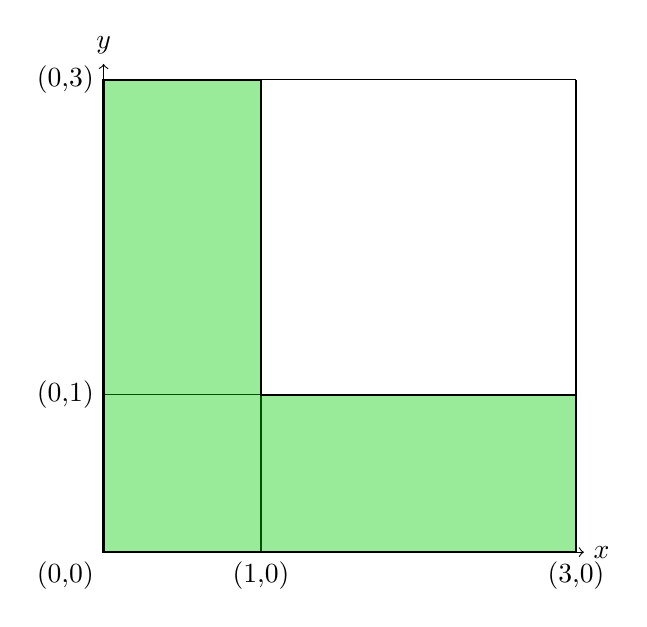
\begin{tikzpicture}
          \draw[->] (0,0) -- (6.1,0) node[right] {$x$};
          \draw[->] (0,0) -- (0,6.2) node[above] {$y$};
          \node[below] (all) at (6,0) {(3,0)};
          \node[left] (all) at (0,6) {(0,3)};
          \node[below left] (all) at (0,0) {(0,0)};

          \node[below] (all) at (2,0) {(1,0)};
          \node[left] (all) at (0,2) {(0,1)};

          \draw (2,0) -- (2,6) node {};
          \draw (0,2) -- (6,2) node {};
          \draw (6,0) -- (6,6) node {};
          \draw (0,6) -- (6,6) node {};
          \filldraw[thick,fill=green!80!black,fill opacity=0.4] (0,0) -- (0,6) -- (2,6) -- (2,2)  -- (6,2) -- (6,0) -- cycle;
        \end{tikzpicture}
        \caption{Het universum}
      \end{figure}
      We zouden dit kunnen uitrekenen als $\int_{0}^{3}\int_{0}^{1}f_{X,Y}(x,y)\ dy dx + \int_{0}^{1}\int_{0}^{3}f_{X,Y}(x,y)\ dy dx - \int_{0}^{1}\int_{0}^{1}f_{X,Y}(x,y)\ dy dx$, maar omdat we eigenlijk niet graag veel integralen uitrekenen kunnen we het eenvoudiger doen door naar te tekening te kijken:
      \[ P(X < 1 \cup Y < 1) = 1 - \int_{1}^{3}\int_{1}^{3}f_{X,Y}(x,y)\ dy dx \]
      \kunnen{We rekenen dit uit:}
      \begin{align*}
        \int_{1}^{3}\int_{1}^{3}f_{X,Y}(x,y)\ dy dx 
        &= \int_{1}^{3}\int_{1}^{3}c(x+y)\ dy dx\\
        &= c\int_{1}^{3}\left.\left(xy+\frac{y^{2}}{2}\right)\right|_{y=1}^{y=3}\ dx\\
        &= c\int_{1}^{3}\left(3x + \frac{9}{2} - x - \frac{1}{2}\right)\ dx\\
        &= c\int_{1}^{3}(2x + 4)\ dx\\
        &= c\left.\left(x^{2} + 4x\right)\right|_{x=1}^{x=3}\\
        &= c\left(9 + 12 - 1 - 4\right)\\
        &= 16c
      \end{align*}
      Het antwoord is dus $P(X < 1 \cup Y < 1) = 11c$.

    \item \kennen{We berekenen de marginale dichtheidsfunctie als volgt:}
      \[ f_{Y|X}(y|x) = \frac{f_{X,Y}(x,y)}{f_{X}(x)} \]
      De teller kennen we al, \kennen{de noemer berekenen we als volgt:}
      \[ f_{X}(x) = \int_{-\infty}^{+\infty}f_{X,Y}(x,y)\ dy \]
      \begin{align*}
        \int_{-\infty}^{+\infty}f_{X,Y}(x,y)\ dy
        &= \int_{0}^{3}c(x+y)\ dy\\
        &= c\left.\left(xy + \frac{y^{2}}{2}\right)\right|_{y=0}^{y=3}\\
        &= c\left(3x + \frac{9}{2}\right)
      \end{align*}
      We kunnen nu de marginale dichtheidsfunctie berekenen:
      \begin{align*}
        \frac{f_{X,Y}(x,y)}{f_{X}(x)}
        &= \frac{c(x+y)}{c\left(3x + \frac{9}{2}\right)}\\
        &= \frac{x+y}{3\left(x+\frac{3}{2}\right)}
      \end{align*}
      Het definitiegebied is $x\in\interval{0}{3}, y\in\interval{0}{3}$.
    \end{enumerate}
  \end{ex-antwoord}
\end{examenvraag}

\end{document}

%%% Local Variables:
%%% mode: latex
%%% TeX-master: t
%%% End:
